\chapter{Conceitos}

\paragraph{}
Ornare arcu odio ut sem nulla pharetra diam sit. Elementum tempus egestas sed sed risus pretium quam. Mauris commodo quis imperdiet massa tincidunt nunc pulvinar sapien. At erat pellentesque adipiscing commodo elit at imperdiet dui. Consectetur purus ut faucibus pulvinar elementum integer. Iaculis nunc sed augue lacus viverra vitae. Cras fermentum odio eu feugiat pretium nibh ipsum. Posuere sollicitudin aliquam ultrices sagittis orci a scelerisque purus. Vulputate ut pharetra sit amet aliquam.

\section{Portas Lógicas}

\subsection{AND}

\paragraph{}
Porta lógica AND (E) (também é chamada de conjunção lógica) é uma operação lógica em dois operandos que resulta em um valor lógico verdadeiro somente se todos os operados tem um valor verdadeiro. Equivale a uma multiplicação. Supondo que essa porta lógica tem duas entradas e que em uma entrada A está um bit em nível lógico alto e na outra entrada B um bit em nível lógico baixo, assim: A = 1 e B = 0. A saída S será um bit em nível lógico baixo pois, 1 x 0 = 0, logo S = 0.

\begin{table}[h]
    \centering
    \begin{tabular}{|l|l|l|}
    \hline
    \rowcolor[HTML]{EFEFEF} 
    A & B & A.B \\ \hline
    0 & 0 & 0   \\ \hline
    0 & 1 & 0   \\ \hline
    1 & 0 & 0   \\ \hline
    1 & 1 & 1   \\ \hline
    \end{tabular}
\end{table}

\subsection{NAND}
\begin{wrapfigure}{l}{0.15\textwidth}
    \centering
    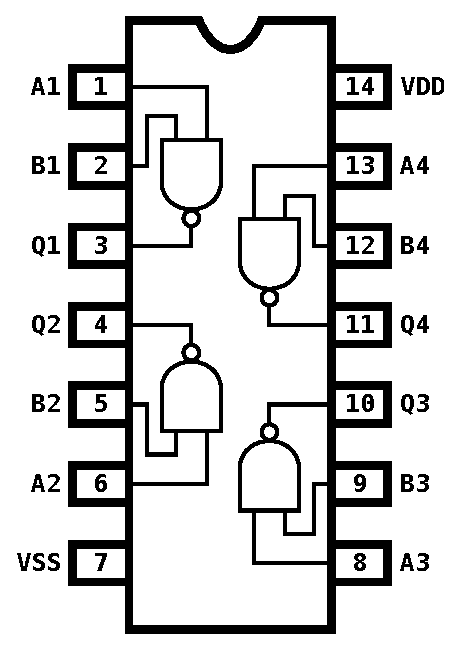
\includegraphics[width=0.15\textwidth]{CMOS_4011_diagram.eps}
\end{wrapfigure}

NAND ou Conectivo de Sheffer é um conectivo utilizado em lógica. Esse conectivo equivale à negação da conjunção, expressa usualmente como "não (algo)... e (algo)... ". Também conhecido como conectivo da negação alternativa, é verdadeiro se pelo menos um dos operandos for falso. No âmbito da álgebra booleana e na eletrônica digital é conhecido como NAND ("não...e..."). É um dos operadores que, por si só, pode ser usado para expressar todas as funções booleanas que podem ser escritas na lógica proposicional. Juntamente com o NEM, é um dos dois operadores unários funcionalmente completos da lógica proposicional. Esse diagrama esquemático mostra como as portas NAND estão arranjadas na parte interna de um circuito integrado CMOS 4011.

\newpage
\section{Exemplo de Código-Fonte de uma operação AND em Arduíno}

\begin{lstlisting}[frame=trbl]
    // se ambos os switches estiverem alimentados
    if (digitalRead(2) == HIGH && digitalRead(3) == HIGH) {
        // statements
    }
\end{lstlisting}